%*******************************************************************************
%****************************** Secondo capitolo *********************************
%*******************************************************************************

\chapter{Lavoro svolto}

\section{Localizzazione}
\label{localizzazione}
L'obiettivo principale di questo lavoro consisteva nella sintesi di un sistema di localizzazione capace di sfruttare in modo complementare il sensore Lidar ed il sistema Pozyx\textsuperscript\textregistered\hspace{1mm}al fine di ottenere un robot capace di localizzarsi in modo affidabile all'interno di una mappa preacquisita. Il problema da risolvere è quello tipico di ogni sistema che sfrutta la tecnologia lidar affiancata ad un filtro a particelle per la localizzazione: infatti, possono verificarsi casi in cui l'insieme di stati probabili non si concentra a sufficienza, casi in cui si evidenziano più zone equiprobabili causando un'indeterminazione non facilmente risolvibile, e casi in cui l'assenza di punti di riferimento validi si traduce nella totale incapacità di percepire spostamenti. L'unico modo di risolvere tali problematiche è quello di "suggerire" all'algoritmo la posa approssimata, anche con varianza "grande", affinché il filtro a particelle concentri la nuvola di stati probabili circa nella giusta posizione.

\subsection{Lidar}
\label{lidar}

Il Lidar si è rivelato essere il sensore più affidabile a disposizione, sia per quanto riguarda l’accuratezza dei risultati, sia per quanto riguarda la percentuale di fallimenti, che è prossima allo zero.

Basandosi su questo presupposto e sull’approccio utilizzato nel progetto precedente, l’utilizzo del Lidar è stato il punto di partenza del lavoro.

L’algoritmo di localizzazione designato è l’Adaptive Monte Carlo Localization (AMCL) descritto nell'Appendice~\ref{appendice1.1}.

\bigskip

Nelle condizioni in cui il robot è stato ricevuto, l’algoritmo non produceva risultati soddisfacenti, il match con la mappa era scarso e di conseguenza anche la localizzazione del veicolo su di essa. 

Effettuando un'analisi approfondita del flusso di dati del sistema, è stato appurato che la causa principale di una localizzazione poco accurata risiedeva nella fonte dell'odometria, necessaria ad AMCL sotto forma di \verb!tf! per funzionare correttamente; questa era ottenuta dai dati di posa provenienti dal sistema UWB, le cui scarse performance si riflettevano in una odometria di altrettanto scarsa qualità.
Ripartendo dunque da un AMCL in versione originale, effettuando tuning su alcuni dei suoi parametri e optando per il nodo \verb!laser_scan_matcher! che utilizza il Lidar stesso come sorgente di odometria, il risultato è notevolmente migliorato rispetto a quello precedente.
Infatti, osservando il robot tramite \verb!Rviz!, partendo da una posa iniziale caratterizzata da una certa covarianza, è sufficiente uno spostamento di poche decine di centimetri per arrivare a convergenza. 

\bigskip

I parametri modificati sono mostrati in Tabella~\ref{table:parametri_amcl_modificati}.

\bigskip
%%%%%%%%%%%%%
\begin{table}[h]
\footnotesize
\caption{Parametri AMCL modificati}
\centering
\label{table:parametri_amcl_modificati}
\begin{tabular}{p{0.2\textwidth}p{0.1\textwidth}p{0.13\textwidth}p{0.3\textwidth}}
\toprule
Parametro           & Default & Modificato & Descrizione \\
\midrule
\texttt{kld\_err}      & $0.01$  & $0.03$     & Massimo errore tra la vera distribuzione e quella stimata.\\

\texttt{laser\_z\_hit}  & $0.95$  & $0.99$     & Peso della parte \texttt{z\_hit} del modello.\\

\texttt{laser\_z\_rand} & $0.05$  & $0.01$     & Peso della parte \texttt{z\_rand} del modello.\\

\texttt{update\_min\_d} & $0.2$   & $0.05$     & Movimento traslazionale richiesto prima di eseguire un aggiornamento del filtro.\\ 

\texttt{update\_min\_a} & $\pi/6$ & $0.01$     &  Movimento rotatorio necessario prima di eseguire un aggiornamento del filtro.\\ 

\bottomrule
\end{tabular}
\end{table}
%%%%%%%%%%%%%%

\bigskip

Tuttavia, nonostante i buoni risultati in condizioni di funzionamento normali, cioè con robot che naviga all’interno di una stanza della quale è disponibile la mappa e nessun tipo di interferenza con il sensore Lidar, ciò che si desidera è rendere la localizzazione robusta ad eventuali perturbazioni o fallimenti.
Infatti, nel caso in cui il sensore Lidar non riuscisse ad effettuare scansioni per un certo intervallo di tempo, oppure sbagliasse la localizzazione del robot a causa di errori nel matching della mappa, si rende necessario un meccanismo che si accorga di tale errore e che intervenga per correggerlo.
Tale meccanismo, che verrà approfondito nel paragrafo \ref{localizzazione_robusta}, è stato messo a punto sfruttando le informazioni provenienti dalle UWB per mandare dei fix di posa quando vi è un'eccessiva differenza rispetto alle stime di posizione di AMCL, scegliendo quella fornita dalle UWB come base su cui reinizializzare il filtro.

\subsection{UWB}
\label{uwb}

La prima cosa da fare per sfruttare le UWB, dopo averle posizionate in un nuovo setup, è attivare la procedura di autocalibrazione, in modo che le ancore si identifichino automaticamente e calcolino le distanze l’una dall’altra. 
Ciò può esser fatto tramite il bash script \verb!./autocalibration.sh! che una volta terminato, oltre a settare in modo corretto le ancore, mostra a schermo l'esito della procedura, in modo da poter valutare la bontà dei risultati. Per eventuali approfondimenti fare riferimento a Crosato-Tesconi\cite{REPORT:1}.

\bigskip

Conclusa la fase di setup e calibrazione inziale, è possibile sfruttare i dispositivi Pozyx\textsuperscript\textregistered\hspace{1mm}connessi al sistema tramite dei nodi dedicati, essenzialmente publisher di posa. Per lo sviluppo di questa parte del software si è deciso di partire dagli scripts Python messi a disposizione dalla Pozyx\textsuperscript\textregistered\hspace{1mm}(\cite{WEBSITE:1}) e di adattarli poi in base alle esigenze del progetto: sono stati realizzati vari nodi che pubblicano la posa delle tag (posizione+quaternione) e le relative \verb!tf!. Dato il rumore presente, è stata implementata la possibilità di filtrare i dati ottenuti dalle tag con filtri a media mobile, tuttavia si sconsiglia di utilizzarli, vista l’introduzione di un ritardo. Inoltre, è da sottolineare che l'utilizzo della media semplice è molto sensibile alla presenza di outliers che sono stati osservati frequentemente durante la conduzione degli esperimenti.

Per approfondimenti sui nodi fare riferimento ad Appendice~\ref{appendice2}.

\bigskip 

Fin dai primi test è sempre emersa una certa inaffidabilità delle tag come principale sistema di localizzazione, poiché pubblicano dati fin troppo rumorosi ed sono soggette a improvvisi fallimenti.

Ad oggi sono state identificate e risolte due possibili cause: per quanto riguarda la prima, si trattava di un tag difettoso che è stato sostituito, mentre la seconda era una forte interferenza elettromagnetica proveniente dall’alimentazione e relativa parte switching, che è stata arginata racchiudendo la parte switching all’interno di un box metallico e spostando la batteria al livello inferiore del robot.

E’ stato predisposto anche un foglio di alluminio che può essere posizionato come ulteriore strato isolante, ma non è sembrato portare alcun tipo di beneficio.

Nonostante le soluzioni adottate, i dati che si ricevono continuano ad essere non precisi e di conseguenza non utilizzabili in modo continuo per una localizzazione affidabile.
Per questo motivo si è deciso di sfruttare il sistema UWB parallelamente ai risultati dello scan matching, utilizzando il dato di posa solo per effettuare un fix di posizione quando vi è una differenza superiore ad $1.5$m rispetto a quella fornita da AMCL (vedi paragrafo \ref{localizzazione_robusta}).

\clearpage

% ********************* SECTION COMUNICAZIONE SERIALE

\section{Comunicazione seriale}
\label{comunicazione_seriale}
Il sistema che si occupa della comunicazione seriale è stato parzialmente riscritto per ottenere maggiore chiarezza e ordine. Lo scopo è quello di gestire il canale di comunicazione tra Intel\textsuperscript\textregistered Joule\texttrademark\hspace{1mm}ed STM\textsuperscript\textregistered\hspace{1mm}per lo scambio reciproco di dati attraverso le porte seriali. L'Intel\textsuperscript\textregistered Joule\texttrademark, funge da raccordo con l'ambiente ROS leggendo e scrivendo su topic accessibili dal resto del sistema, mentre l'STM\textsuperscript\textregistered\hspace{1mm}crea una connessione con lo schematico Simulink\textsuperscript\textregistered\hspace{1mm}su di essa implementato. 

\bigskip

\begin{figure}[h] 
\centering    
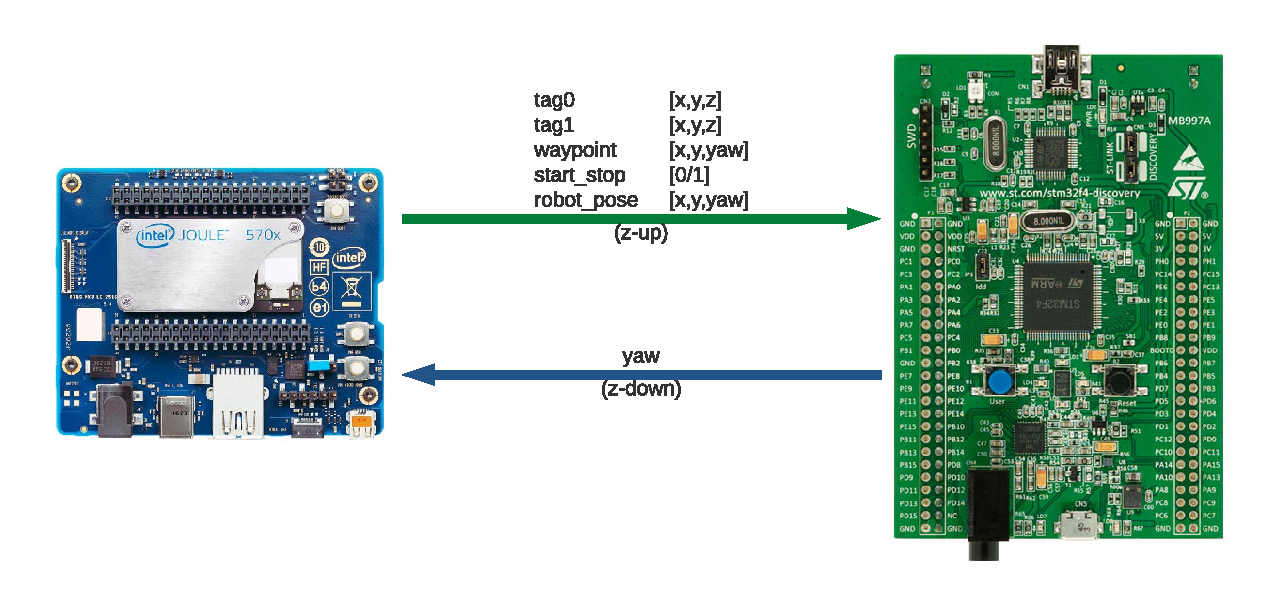
\includegraphics[width=1\textwidth]{Capitolo2/Figs/schema_tattico.pdf}
\caption[Schema comunicazione seriale]{Schema comuncazione seriale}
\label{fig:schema_serialcom}
\end{figure}

\bigskip

I dati necessari per la localizzazione vengono raccolti a livello dell'Intel\textsuperscript\textregistered Joule\texttrademark\hspace{1mm}, che procede quindi ad elaborarli ed in seguito inviarli alla scheda a valle (STMF407\textsuperscript\textregistered) insieme al goal da raggiungere\footnote{impostabile tramite Rviz con il comando \texttt{2DNavGoal} oppure pubblicando sul topic \texttt{/waypoint\_publisher}}.
L’STM\textsuperscript\textregistered, sulla base dei dati ricevuti, calcola il controllo da dare ai motori per raggiungere l’obiettivo impostato; parallelamente a ciò misura costantemente l'heading del veicolo inviandolo all'Intel\textsuperscript\textregistered Joule\texttrademark\hspace{1mm}.

I dati scambiati sono riassunti nelle Tabelle~\ref{table:comunicazione_seriale2stm}\ref{table:comunicazione_stm2seriale}.

\bigskip
\bigskip

\begin{savenotes}
\begin{table}[h]
\begin{minipage}{\textwidth}
\renewcommand\thempfootnote{\arabic{mpfootnote}}
\footnotesize
\caption{Comunicazione seriale Intel\textsuperscript\textregistered Joule\texttrademark\hspace{1mm}$\rightarrow$ STM32\textsuperscript\textregistered}
\centering
\label{table:comunicazione_seriale2stm}
\begin{tabular}{lll}
\toprule
Nome                 & Descrizione                                & Dimensione\\
\midrule
\verb!HEADER_A!      & 0x1A                                       & 1 Byte\\
\verb!HEADER_B!      & 0x1B                                       & 1 Byte\\
\verb!PAYLOAD!       & 0x2C                                       & 1 Byte\\
\hline
\verb!pos_x_f!       & tag $0$ - coordinata $x$ - frame UWB       & 4 Byte\footnote{float}\\
\verb!pos_y_f!       & tag $0$ - coordinata $y$ - frame UWB       & 4 Byte\textsuperscript{2}\\
\verb!pos_z_f!       & tag $0$ - coordinata $z$ - frame UWB       & 4 Byte\textsuperscript{2}\\
\hline
\verb!pos_x_b!       & tag $1$ - coordinata $x$                   & 4 Byte\textsuperscript{2}\\
\verb!pos_y_b!       & tag $1$ - coordinata $y$                   & 4 Byte\textsuperscript{2}\\
\verb!pos_z_b!       & tag $1$ - coordinata $z$                   & 4 Byte\textsuperscript{2}\\
\hline
\verb!way_x!         & waypoint - coordinata $x$ - frame map    & 4 Byte\textsuperscript{2}\\
\verb!way_y!         & waypoint - coordinata $y$ - frame map    & 4 Byte\textsuperscript{2}\\
\verb!way_z!         & waypoint - $yaw$  - frame map            & 4 Byte\textsuperscript{2}\\
\hline
\verb!start_stop!    & $0 = disabilita\ motori$ | $1 = abilita\ motori$       & 4 Byte\textsuperscript{2}\\
\hline
\verb!robot_pose_x!  & posa stimata da AMCL - coordinata x - frame map   & 4 Byte\textsuperscript{2}\\
\verb!robot_pose_y!  & posa stimata da AMCL - coordinata y - frame map   & 4 Byte\textsuperscript{2}\\
\verb!robot_pose_z!  & posa stimata da AMCL - yaw - frame map            & 4 Byte\textsuperscript{2}\\

\bottomrule
\end{tabular}
\end{minipage}
\end{table}
\end{savenotes}

I primi tre elementi sono header che codificano il tipo di messaggio, mentre i restanti sono informazioni utili che verranno lette ed interpretate. 

In dettaglio, le coordinate delle due tag vengono utilizzate dall'STM\textsuperscript\textregistered\hspace{1mm} per misurare lo yaw del veicolo\footnote{L'angolo è misurato rispetto all'asse $x$ del frame \texttt{UWB}, riportandolo poi in un sistema di riferimento $z-down$}, che insieme alla posa stimata da AMCL, ed al waypoint impostato, sono sfruttate per determinare il controllo dei motori. Infine l'elemento \verb!start_stop! (booleano) li abilita o disabilita.

Il valore dello $yaw$ è inviato dall'STM\textsuperscript\textregistered\hspace{1mm}in un pacchetto come quello mostrato in Tabella~\ref{table:comunicazione_stm2seriale}.

\bigskip
\bigskip

\begin{table}[h]
    \footnotesize
    \caption{Comunicazione STM32\textsuperscript\textregistered\hspace{1mm}$\rightarrow$ seriale Intel\textsuperscript\textregistered Joule\texttrademark}
\centering
\label{table:comunicazione_stm2seriale}
\begin{tabular}{lll}
\toprule
Nome                     & Descrizione   & Dimensione\\
\midrule
\verb!HEADER_A!          & 0x1A          & 1 Byte\\
\verb!HEADER_B!          & 0x1B          & 1 Byte\\
\verb!PAYLOAD_POSE!      & 0x2C          & 1 Byte\\
\hline
\verb!yaw!               & $yaw$         & 4 Byte\\
\bottomrule
    \end{tabular}
\end{table}

\subsection{Problematiche}
A seguito della prima prova sperimentale in cui si chiedeva al robot di portarsi da una punto di partenza ad uno di arrivo, si è osservato un malfunzionamento del sistema: non appena i motori venivano abilitati, il servo iniziava ad avere un comportamento anomalo variando continuamente tra l'orientazione corretta e la posizione di riposo. Questo tipo di comportamento comprometteva la possibilità di portare a termine test e verifiche sul software sviluppato. Sicuramente il difetto era presente anche nel sistema originale consegnato insieme al robot, tuttavia, le problematiche presenti a monte del controllo lo avevano mascherato impedendone l'identificazione prima della loro soluzione, poiché sembravano esserne la causa.

Si è resa quindi più che necessaria l’identificazione della sorgente del problema. 
\bigskip

La ricerca è avvenuta in più passi, con lo scopo di restringere volta per volta il malfunzionamento ad un’area sempre più circoscritta:

\begin{itemize}
    \bigskip
    \item \textbf{Test 1} - isolamento del controllo: in questa prova è stato testato il corretto funzionamento di tutti i motori (anteriore, posteriore e servo) connettendoli direttamente ad un segnale PWM noto generato con un Arduino\textsuperscript\textregistered, con andamento ad onda triangolare. Il test ha avuto esito positivo restringendo la zona in cui cercare il difetto alla coppia Intel\textsuperscript\textregistered Joule\texttrademark\hspace{1mm}ed STM\textsuperscript\textregistered\hspace{1mm}ed alla loro connessione e comunicazione;
    \bigskip
    \item \textbf{Test 2} - controllo dei dati provenienti dalla Intel\textsuperscript\textregistered Joule\texttrademark\hspace{1mm}: in questa prova è stato chiuso su se stesso il sistema di comunicazione seriale dell’Intel\textsuperscript\textregistered Joule\texttrademark\hspace{1mm}connettendo il canale di trasmissione a quello di ricezione ed osservando i dati ricevuti. Anche questo test ha avuto esito positivo escludendo la scheda dalle possibili sorgenti del malfunzionamento;
    \bigskip
    \item \textbf{Test 3} - controllo ricezione seriale STM\textsuperscript\textregistered: in questa prova si è voluto verificare che il problema non fosse la comunicazione seriale tra Intel\textsuperscript\textregistered Joule\texttrademark\hspace{1mm}e STM\textsuperscript\textregistered, generando gli stessi messaggi che sarebbero stati prodotti dall'Intel\textsuperscript\textregistered Joule\texttrademark\hspace{1mm}con un Arduino ed inviandoli quindi all’STM\textsuperscript\textregistered. Il servo ha mantenuto il comportamento indesiderato oscillando tra le solite posizioni, confermando di conseguenza che la sorgente del problema risiedeva all’interno dell’STM\textsuperscript\textregistered;
    \bigskip
    \item \textbf{Test 4} - controllo dei segnali in uscita dall’STM\textsuperscript\textregistered: questo test è stato svolto mantenendo Arduino\textsuperscript\textregistered\hspace{1mm}come sorgente del messaggio seriale contenente dati costanti, a cui dovrebbe corrispondere un controllo costante. I due segnali PWM di controllo dei motori sono stati dunque intercettati ed analizzati tramite un oscilloscopio digitale, grazie al quale è stato possibile osservare una variazione sul tempo di livello alto del segnale in ingresso al servo.
    I due valori di “tempo alto” osservati e mostrati in Figura~\ref{fig:oscilloscopio}, codificano esattamente la posizione di estrema rotazione verso destra ($2.21$ms) e quella di riposo centrale ($1.54$ms) descritte in precedenza.  Figura~\ref{fig:oscilloscopio};
    \bigskip
    \item \textbf{Test 5} - controllo dei segnali in uscita dall’STM\textsuperscript\textregistered\hspace{1mm}a livello dello schematico Simulink\textsuperscript\textregistered: stabilito che la causa del malfunzionamento era da imputarsi al software implementato nell'STM\textsuperscript\textregistered, è stato modificato il punto di ingresso dei dati nello schematico predisponendolo a leggere dalla porta USB di un computer alla quale connettere Arduino\textsuperscript\textregistered. Lo schematico è mostrato in Figura~\ref{fig:modifica schematico Simulink}: è stato inserito un subsystem per interfacciare lo streaming dei dati sulla porta seriale, costituito da pacchetti di $52$ byte, con la restante parte del sistema che si aspetta 13 elementi da $4$ byte ciascuno.  Eseguendo quindi la simulazione su computer è stato possibile andare ad analizzare, uno ad uno, i valori dei vari segnali presenti, cercando il punto in cui avveniva la corruzione dei dati. L'analisi condotta non ha portato a risultati tangibili mostrando un'apparente corretto funzionamento del sistema.
    
\end{itemize}
\clearpage



\begin{figure}[h]
\centering
\hfill
\subfloat[Misura 1: Tempo $2.21$ms]{
	\label{subfig:oscilloscopio1}
    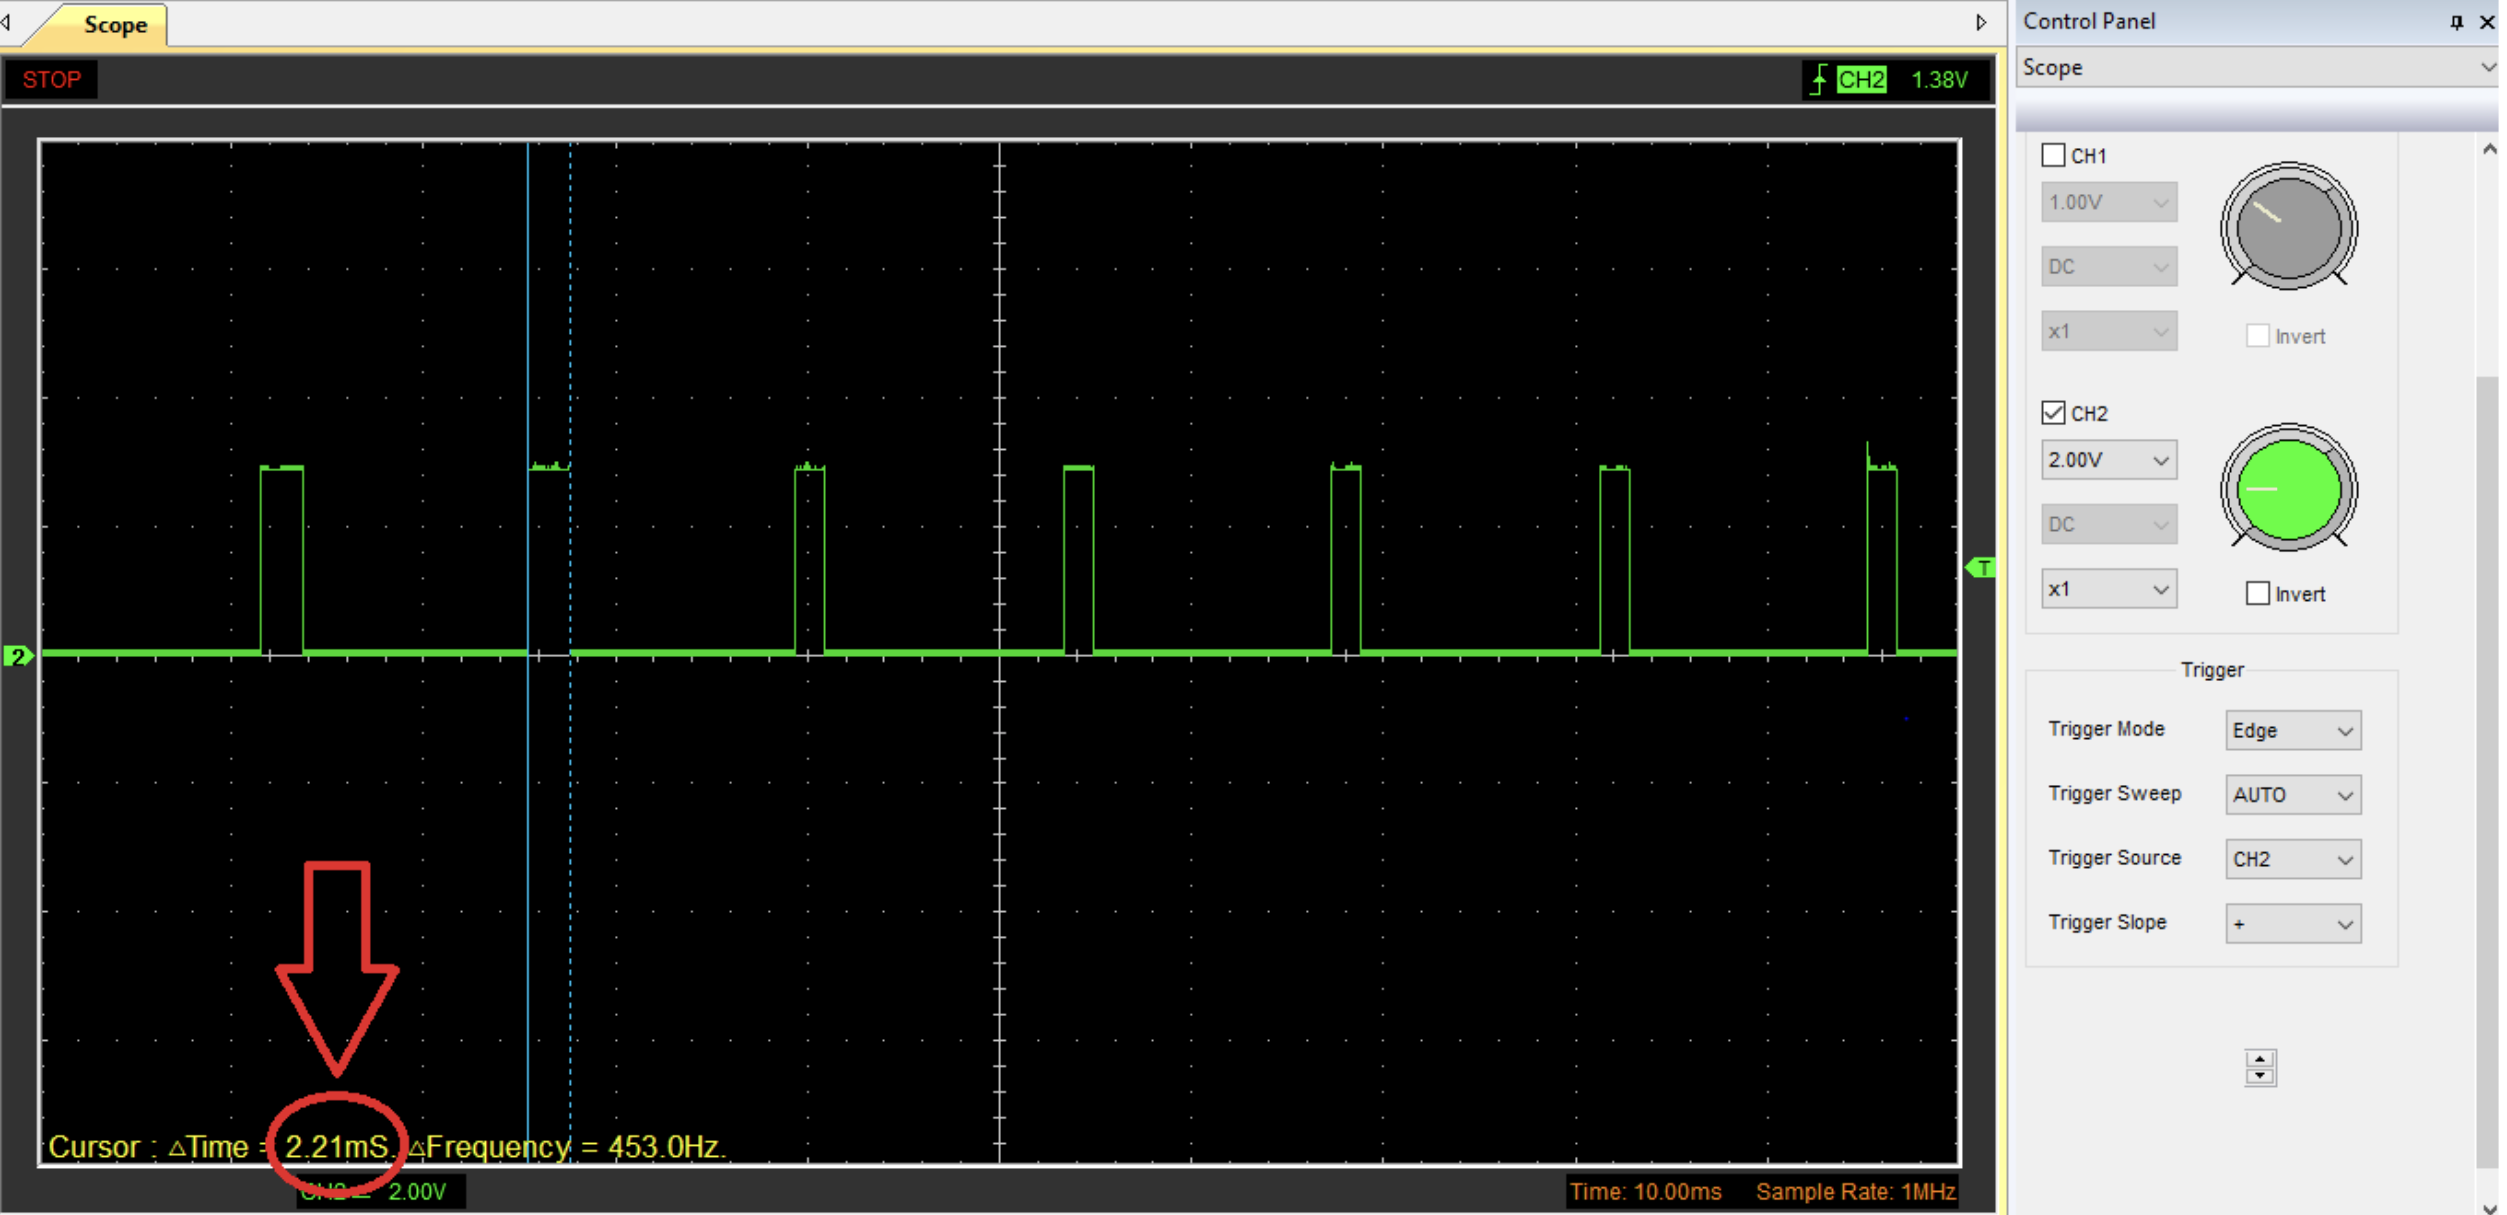
\includegraphics[width=1\textwidth]{Capitolo2/Figs/test4_1.png} } 

\subfloat[Misura 2: Tempo $1.54$ms]{
	\label{subfig:oscilloscopio2}
	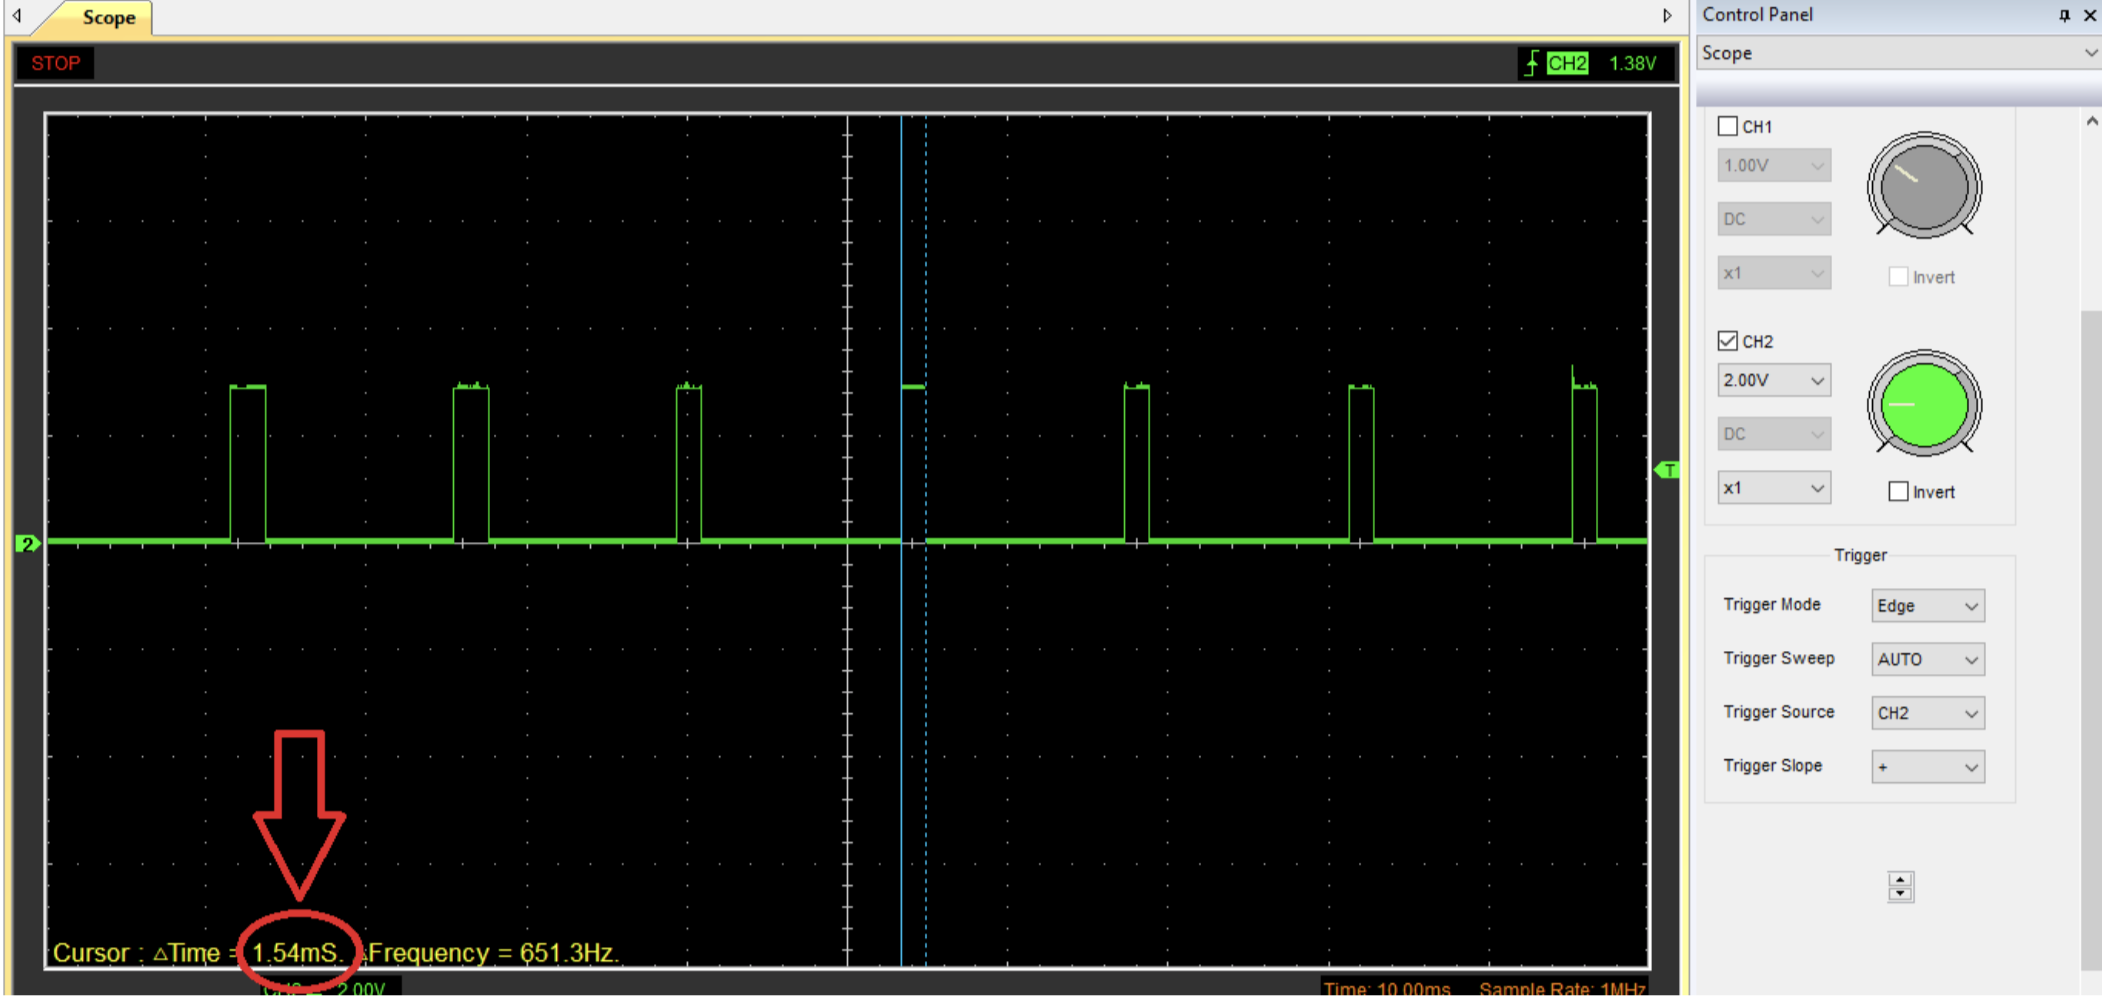
\includegraphics[width=1\textwidth]{Capitolo2/Figs/test4_2.png} } 

\caption{Misura tempo alto con oscilloscopio}
\label{fig:oscilloscopio}
\hspace*{\fill}
\end{figure}


\clearpage

\begin{figure}[h]
\centering
\hfill
\subfloat[Punto di modifica dello schematico]{
	\label{subfig:subsystem}
	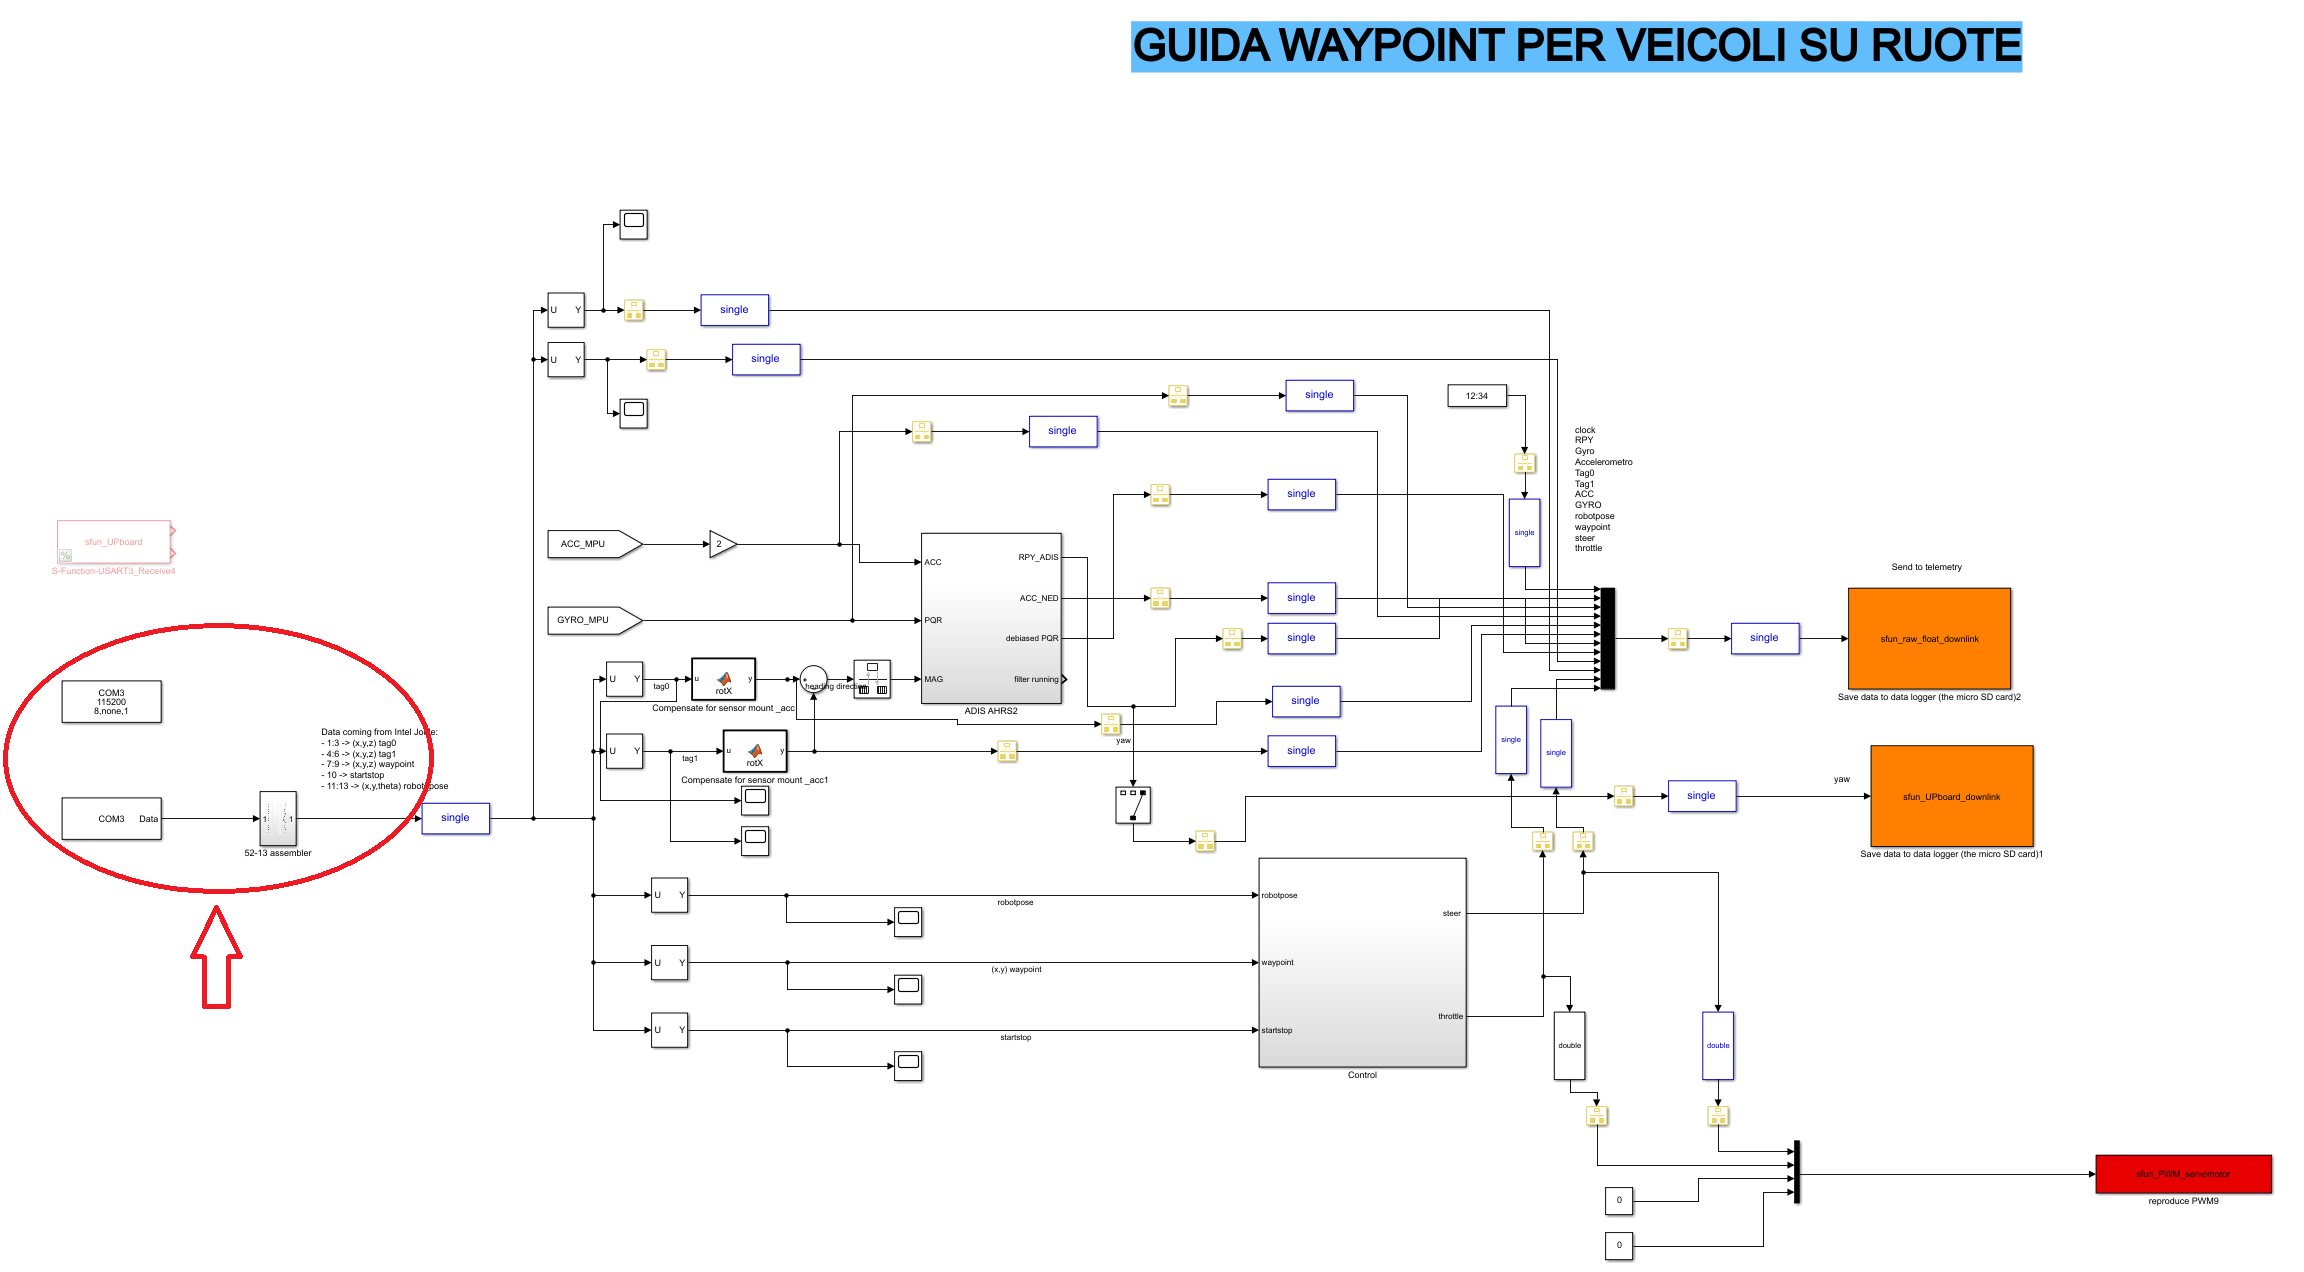
\includegraphics[width=.8\textwidth]{Capitolo2/Figs/test5_1.png} } 
	
\subfloat[Dettaglio del subsystem]{
	\label{subfig:dettaglio del subsystem}
	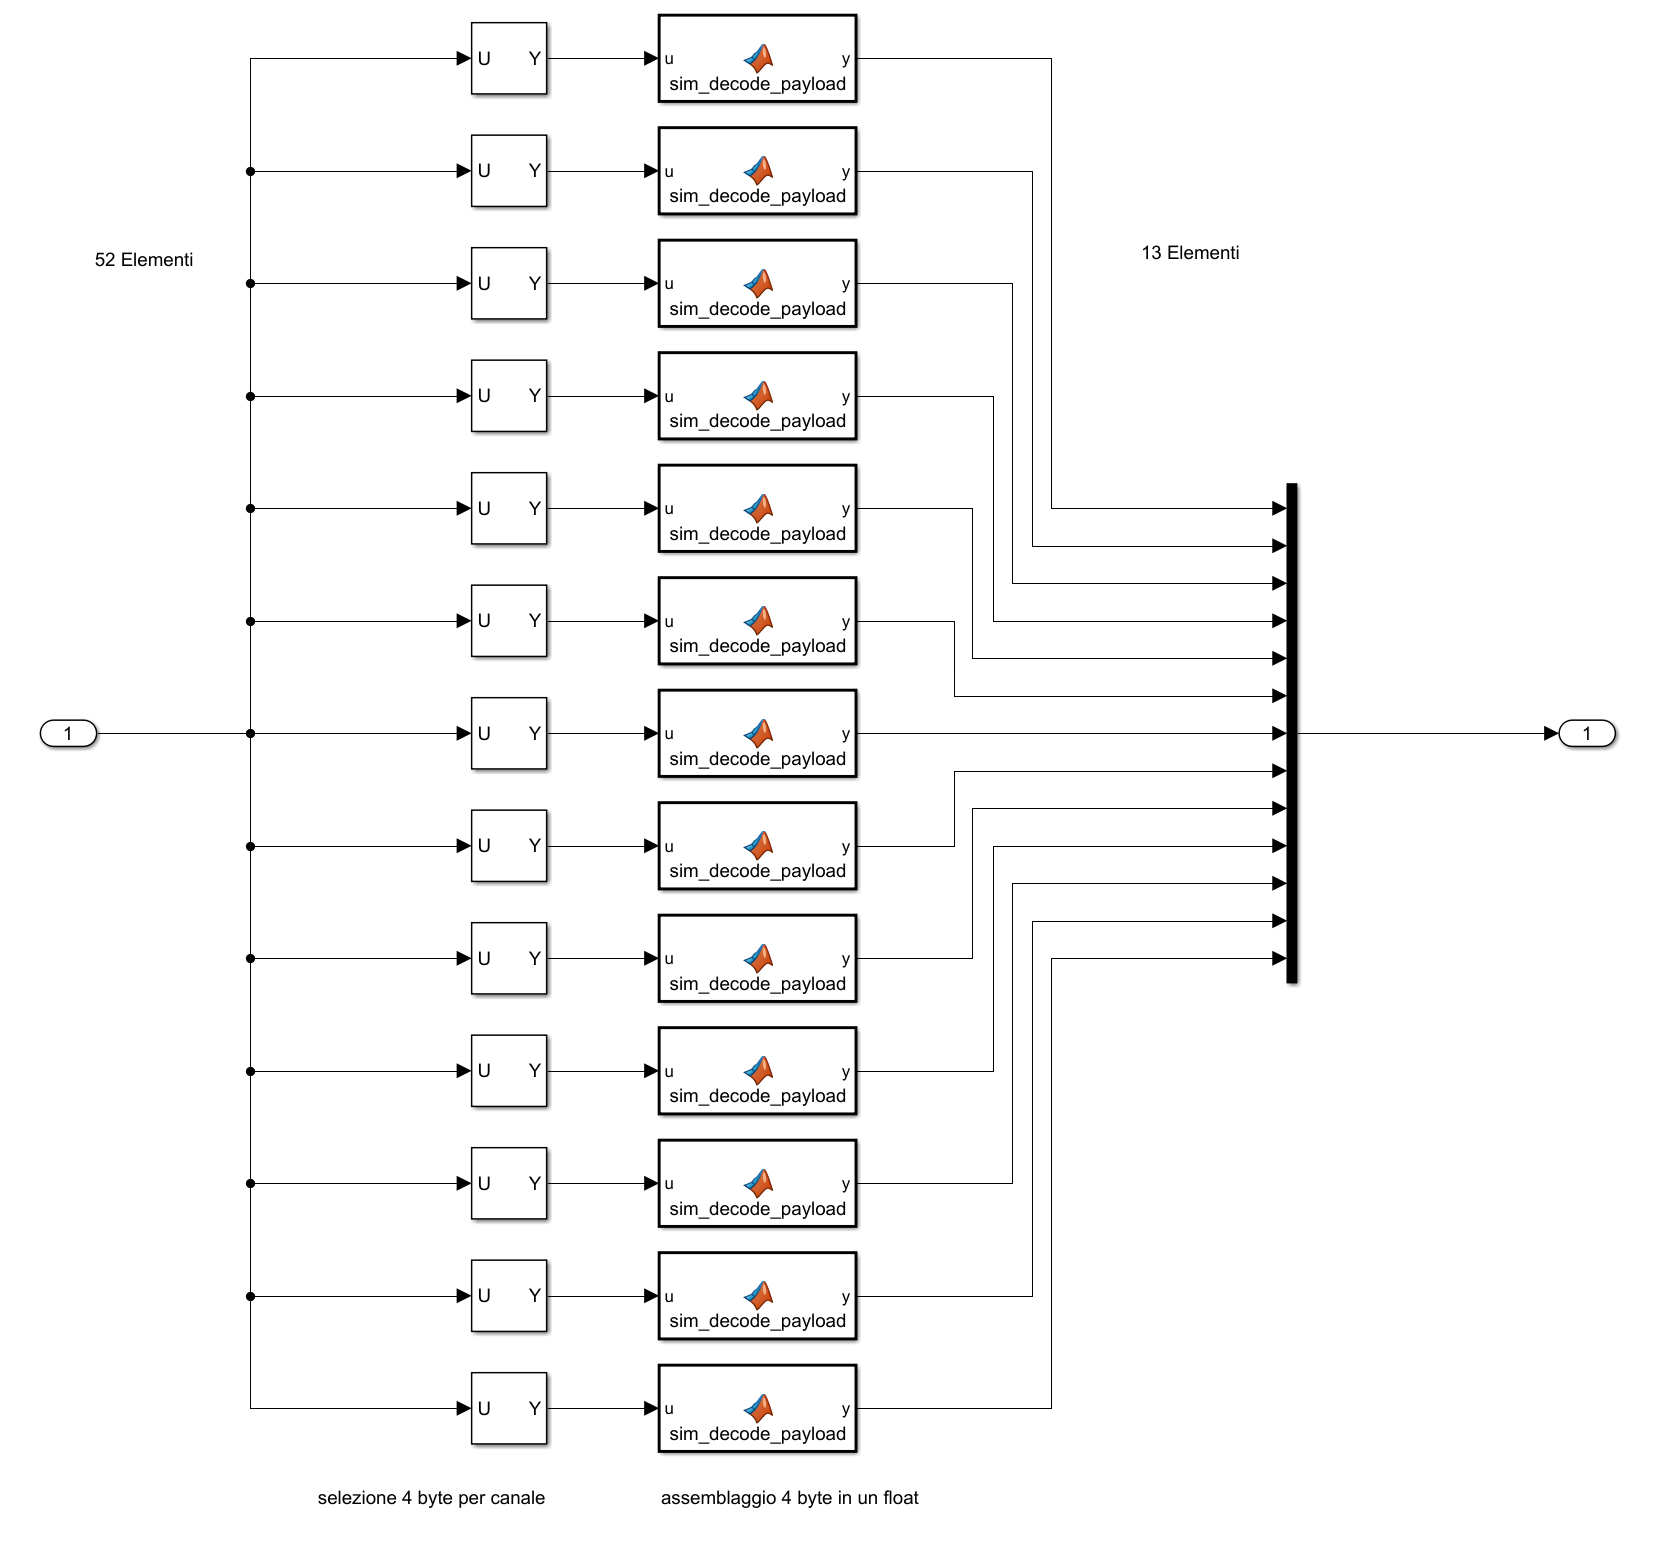
\includegraphics[width=.8\textwidth]{Capitolo2/Figs/test5_2.png} } 

\caption[Modifica schematico Simulink per connessione Arduino e simulazione su PC]{Modifica schematico Simulink per connessione Arduino e simulazione su PC}
\label{fig:modifica schematico Simulink}
\hspace*{\fill}
\end{figure}

\clearpage

Poiché la causa del problema è stata localizzata con certezza all’interno dell’STM\textsuperscript\textregistered\hspace{1mm}ma dai test eseguiti non sono state ottenute le risposte desiderate, si è proceduto ad un’indagine ancora più approfondita sullo schematico Simulink\textsuperscript\textregistered\hspace{1mm}in esecuzione sull’STM\textsuperscript\textregistered, andando a ispezionare anche i livelli in cui viene configurato l'hardware. Si è quindi scoperto che il modulo GPS risultava abilitato nonostante non fosse presente e che eseguiva frequenti letture sulla medesima porta seriale utilizzata dal controllo, corrompendone i dati. La disattivazione del modulo GPS ha risolto il problema definitivamente, aprendo la strada a test e sperimentazioni.

\bigskip

Corretti i problemi di comunicazione, è stato possibile analizzare il controllo implementato, che si è rivelato migliorabile: il sistema di controllo presente per l’acceleratore presentava più blocchi e in uscita forniva il tempo alto del segnale PWM di controllo semplicemente ponendolo uguale al segnale di errore (in metri) e limitandolo con una saturazione.

\bigskip
\bigskip

\begin{figure}[h] 
\centering    
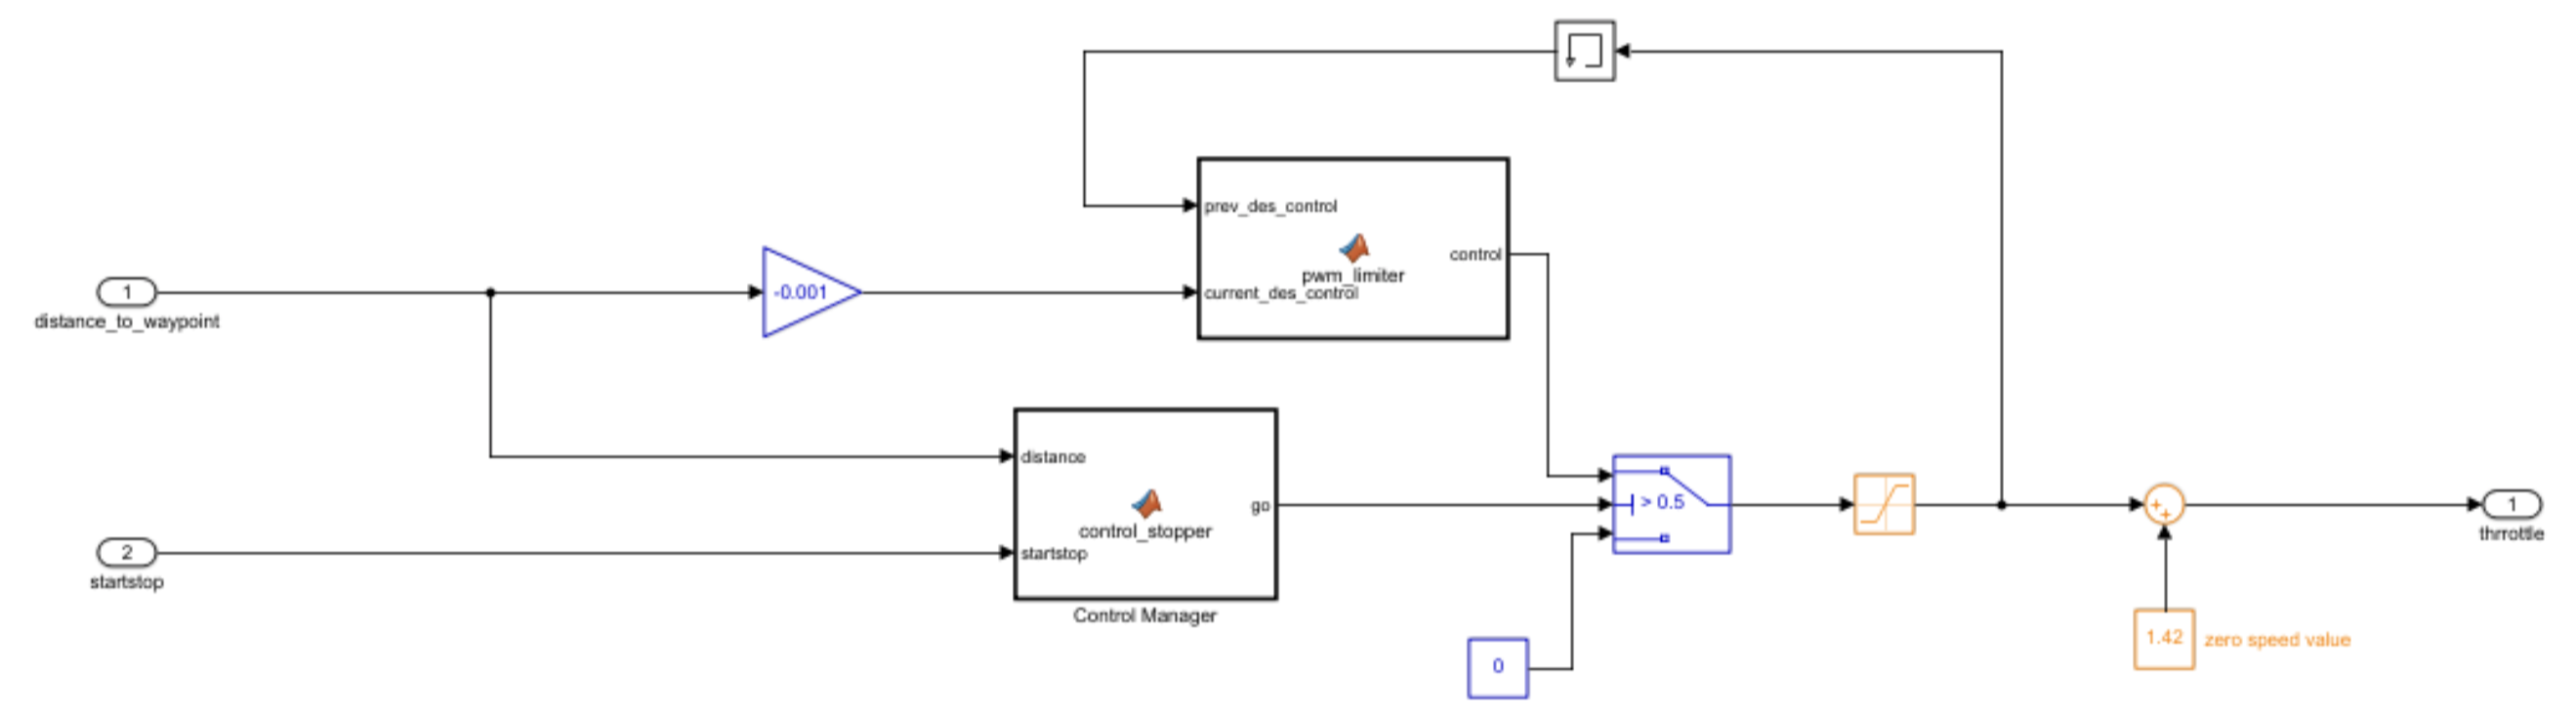
\includegraphics[width=0.9\textwidth]{Capitolo2/Figs/simulink1.png}
\caption[Simulink - controllo iniziale]{Simulink - Controllo iniziale}
\label{fig:controllo_iniziale}
\end{figure}

\bigskip

Tuttavia l’errore non è direttamente traducibile come un valore sensato di PWM ed il sistema di fatto andava sempre a lavorare in saturazione. Per migliorare questo comportamento e per ridurre la complessità del sistema, è stato progettato un nuovo blocco di controllo, unico, che valuta l’errore commesso e restituisce in uscita direttamente un valore di PWM compatibile con il microcontrollore. All’interno del nuovo blocco, l’errore di posizione è comparato con delle soglie che determinano il “grado di lontananza dal goal” e tramite le quali si determina l’ampiezza del controllo da dare ai motori. Per smussare le variazioni a gradino del controllo, è stato aggiunto un polo sull’uscita con costante di tempo di 2 secondi e guadagno unitario; tale filtro è stato disabilitato per non introdurre ritardi sul sistema.

\bigskip
\bigskip

\begin{figure}[h] 
\centering    
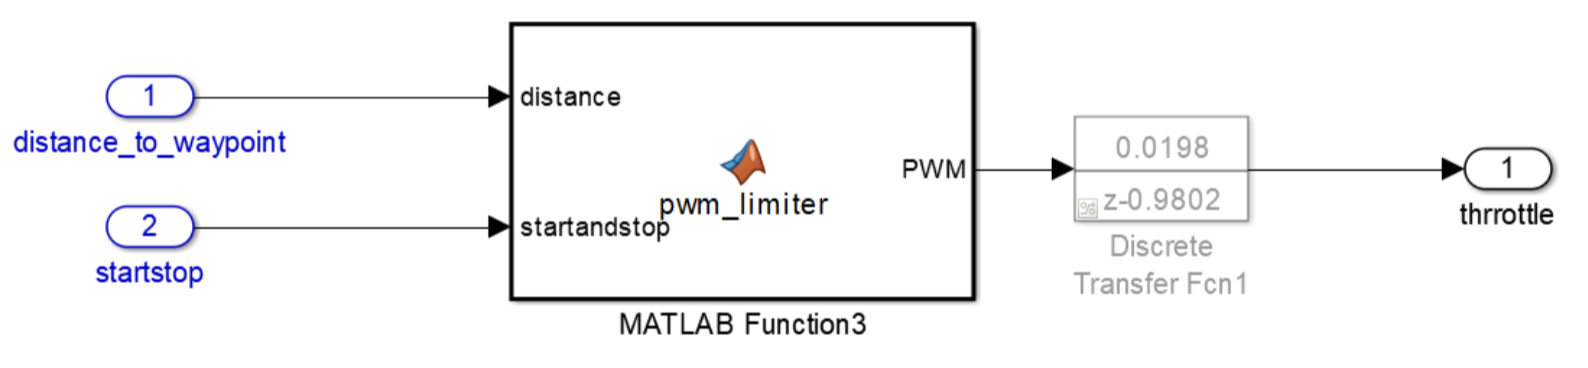
\includegraphics[width=0.9\textwidth]{Capitolo2/Figs/simulink2.png}
\caption[Simulink - controllo finale]{Simulink - Controllo finale}
\label{fig:controllo_finale}
\end{figure}

%********************** SECTION LOCALIZZAZIONE ROBUSTA *************************
\section{Localizzazione robusta}
\label{localizzazione_robusta}

Per rendere robusta la localizzazione tramite il Lidar, è stata implementato un sistema ausiliario che invia dei fix di posa quando la stima fornita da AMCL differisce eccessivamente dalla posizione fornita dal sistema UWB. 

Ciò può accadere principalmente nei seguenti scenari:

\begin{itemize}
    \item Fallimento dello scan matching, cioè quando non si riesce ad associare correttamente le scansioni ricevute alla mappa e di conseguenza la posa inferita da AMCL è errata;

    \item “Kidnapped robot problem”, cioè quando il robot viene forzatamente spostato in una nuova posizione arbitraria oscurando il sensore Lidar in modo che durante lo spostamento non sia in grado di cogliere variazioni nello scan e di conseguenza aggiornare la sua posizione. Quando poi il sensore viene scoperto e la scansione può ripartire, AMCL continuerà a dare come posa stimata quella precedente allo spostamento, nonostante non ci sia più match con la mappa.
\end{itemize}

Questi problemi sono stati risolti sviluppando il nodo \verb!pose_fix_pub! il quale osserva costantemente sia i dati di posa del punto medio tra le tag, sia la stima fornita da AMCL; istante per istante calcola l’errore (in norma 2) tra le due, e qualora questo risulti superiore ad $1.5$m, avvia la procedura di fixing di posa descritta di seguito: 

\begin{enumerate}
    \item Salvataggio della posa del punto medio tra le tag, corrispondente all'incirca alla posizione del Lidar sul robot, con orientazione letta dall'STM\textsuperscript\textregistered; 
    \item Disabilitazione dei motori per motivi di sicurezza - funzione attualmente non attiva
    \item Pubblicazione della posa appena salvata sul topic \texttt{/initialpose} a cui è iscritto AMCL e che ha come effetto una reinizializzazione del filtro nel punto indicato con covarianza pari a quella che si avrebbe all'avvio. A questo punto, il filtro attenderebbe uno spostamento o una rotazione per effettuare un update della stima di posa. L'entità delle variazioni necessarie è specificata nei parametri \texttt{update\_min\_d} (minima traslazione) e \texttt{update\_min\_a} (minima rotazione);
    \item Per forzare il filtro a portare a convergenza la stima riallineandosi con la mappa mentre il robot è fermo, viene effettuata una modifica online del parametro \texttt{update\_min\_d} di AMCL settandolo a zero tramite chiamata al service \texttt{dynamic\_reconfigure} che reinizializzazione il filtro con il parametro scelto;
    \item Attesa, necessaria alla convergenza del filtro;
    \item Nuova chiamata al service \texttt{dynamic\_reconfigure} per riportare il parametro \texttt{update\_min\_d} al valore precedente (questo causa una nuova reinizializzazione del filtro)
    \item Riabilitazione dei motori(se prima erano abilitati) - funzione attualmente non attiva

\end{enumerate}
Lo schema dell'algoritmo è mostrato nella Figura~\ref{fig:fix_posa}.

\begin{figure}[h] 
\centering    
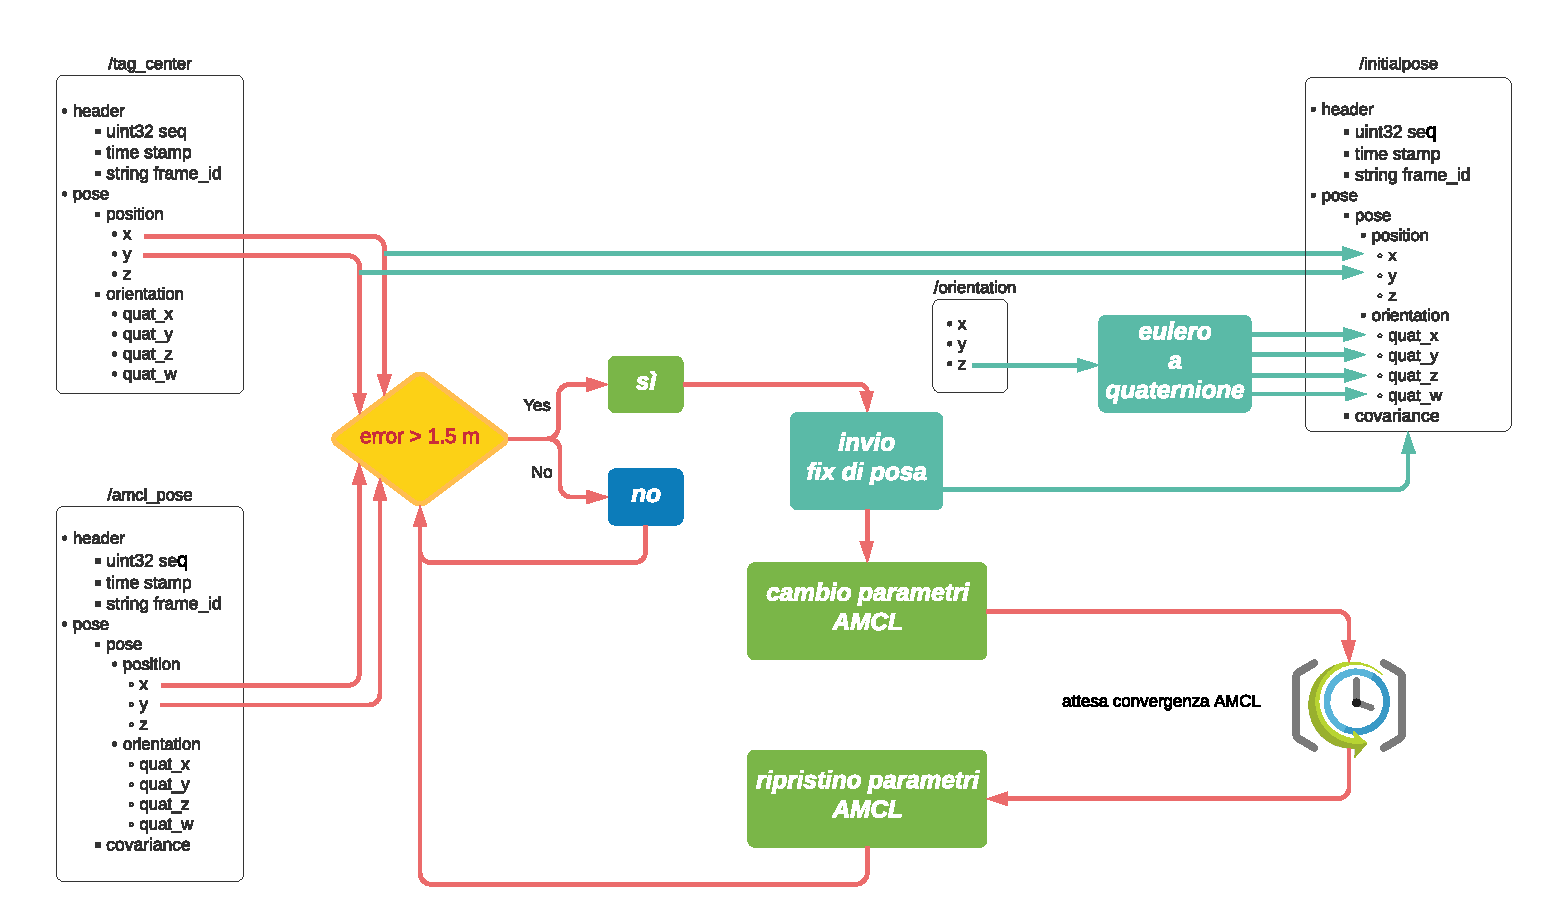
\includegraphics[width=1\textwidth]{Capitolo2/Figs/schema_fix_posa.pdf}
\caption[Fix di posa]{Fix di posa}
\label{fig:fix_posa}
\end{figure}

Il tempo totale per completare una reinizializzazione a seguito di un fix di posa è influenzato da vari fattori: vi è un ritardo fisso di 4s impostato via software per motivi di stabilità\footnote{La procedura di reinizializzazione online di AMCL non ha sempre esito positivo causando talvolta la morte del processo; la frequenza con cui queste reinizializzazioni sono richieste è determinante, richieste troppo ravvicinate hanno sempre condotto a crash di sistema.}, a cui si sommano circa 10-15s necessari ad AMCL per gestire le due reinizializzazioni e convergere (la variabilità è legata alla "bontà" della stima ricevuta, a fix particolarmente buoni corrisponderà un tempo di convergenza ridotto, mentre fix peggiori richiederanno più passi dell'algoritmo per convergere). Nonostante i molteplici tentativi, non è stato possibile ridurre questi tempi di attesa.

\subsection{Oscuramento Lidar}
\label{correzione_oscuramento_lidar}
Quando il Lidar è oscurato, il filtro a particelle (AMCL) non è in grado di fornire alcun update per la stima di posa del robot e di conseguenza non vengono pubblicati messaggi sul topic \texttt{\/robot\_pose} che deriva da \texttt{\/amcl\_pose} e necessario per il controllo dei motori. A livello di interfaccia grafica, ciò corrisponde a vedere invariata la posa del robot su Rviz anche mentre quest'ultimo viene spostato rigidamente. 
Senza ulteriori accorgimenti, finché il Lidar non tornerà online, per via del funzionamento di AMCL, non sarà possibile aggiornare la posa del robot che pertanto rimarrà pari all'ultima disponibile prima dell'oscuramento del sensore. Durante tutto questo intervallo non si avrà alcuna informazione su eventuali spostamenti del robot.

Tornato online il Lidar, AMCL riprenderà a pubblicare ed arriverà anche un fix di posa a causa della discordanza con le UWB e solo a conclusione di questa fase sarà nuovamente disponibile una posa affidabile.

Per avere sempre una traccia degli spostamenti del robot anche nella situazione sopra descritta, si è ideato un procedimento che, osservando i dati provenienti dal Lidar, è in grado di sostituirsi ad AMCL come fonte di dati per \texttt{\/robot\_pose}.

L'elemento chiave è il campo \texttt{intensities} del messaggio\footnote{Di tipo \texttt{LaserScan}} che viene trasmesso sul topic \texttt{\/scan}, il quale è costituito da un array che contiene valori non nulli solo quando il Lidar funziona correttamente. Pertanto, monitorandolo continuamente si è in grado di stabilire quando si hanno malfunzionamenti ed intervenire, sfruttando i dati provenienti dalle UWB come sorgente per \texttt{\/robot\_pose}. Più in dettaglio, si fa riferimento ai messaggi sul topic \texttt{\/tag\_center}, contenenti la posa del punto medio tra le due tag, con orientazione ottenuta dall'STM, i quali sono già riferiti al frame \texttt{map} e quindi coerenti con quelli si avrebbero da AMCL. 


Uno schema di funzionamento di tale sistema è descritto in Figura~\ref{fig:amcl2robotpose}.

\begin{figure}[h] 
\centering    
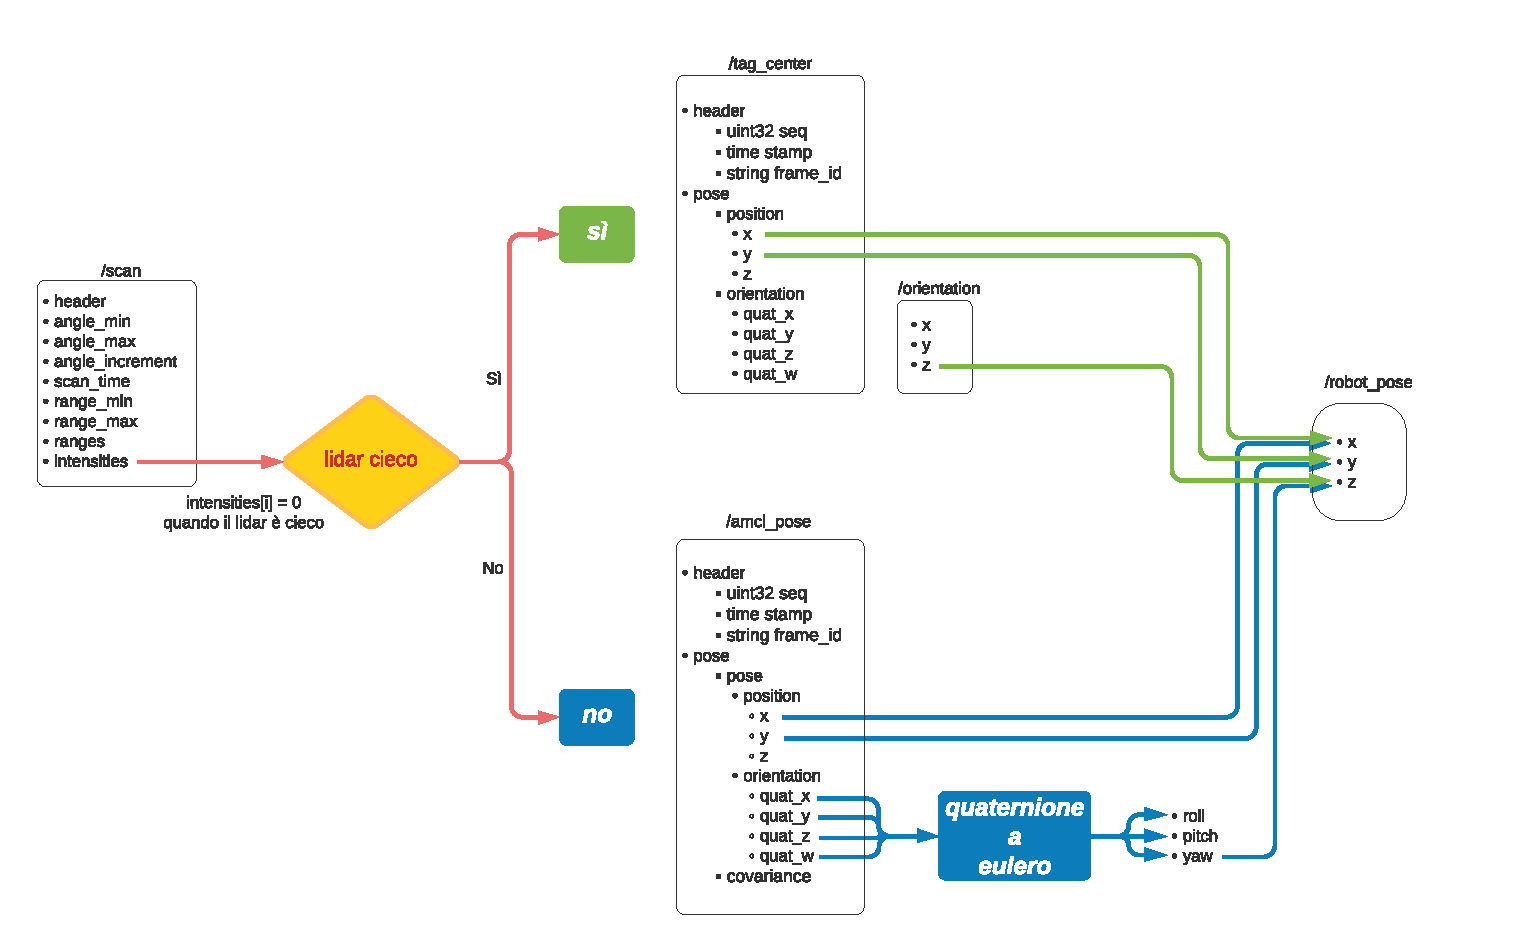
\includegraphics[width=1\textwidth]{Capitolo2/Figs/schema_amcl2robotpose.pdf}
\caption[Schema \texttt{amcl2robotpose}]{Schema \texttt{amcl2robotpose}}
\label{fig:amcl2robotpose}
\end{figure}